\section{\FTMlangGerEng{Aufgabenstellung}{Topic}}%

Autonomous vehicles are rapidly becoming a widespread reality. However, their perception systems still face significant challenges 
in complex and unforeseen scenarios, often leading to disengagements, where human intervention via teleoperation is required. 
In such critical moments, the vehicle must rely on an accurate and robust perception system to ensure safe navigation. 

Most existing perception systems, responsible for detecting and tracking objects in the vehicle's surroundings, rely heavily
on learning-based solutions. While these methods have demonstrated impressive performance in structured and controlled environments, 
they often struggle to generalize in novel and untrained scenarios. This limitation is particularly problematic in safety-critical
situations, where the vehicle must make quick decisions based on the perceived environment.

This project aims to develop a deterministic, stereo camera-based perception system for autonomous vehicles, capable of providing
a reliable and robust understanding of the vehicle's surroundings, even in highly dynamic and unforeseen scenarios. The system
will take as input two images from a stereo camera mounted on the vehicle and output a list of detected objects in the scene, along
with their criticality scores, forming a situational awareness module to assess potential hazards. 
Additionaly, this deterministic approach could run in parallel with existing learning-based perception systems, providing a
an additional layer of redundancy and security in critical situations where the learning-based methods may fail.

To achieve accurate 6D motion estimation (position + velocity), the system will implement a deterministic algorithm 
inspired by the Daimler 6D Vision system. This approach uses Kalman Filters to estimate a 6D state vector for selected feature
points in the scene, which will then be clustered to identify moving objects. Unlike learning-based methods, this approach
does not require extensive training data and can generalize well in new unseen scenarios.

Given the real-time requirements of autonomous vehicles, the system will be implemented in C++ using the Robot Operating System (ROS)
framework. It will also incorporate GPU hardware acceleration using CUDA to speed up computationally intensive tasks, such as
feature point detection, clustering or optical flow computation.  

To ensure scalability and modularity, the entire system will be containerized using Docker, facilitating deployment across different
hardware configurations. Finally, the developed system will be deployed and evaluated on the EDGAR research vehicle. Here, 
the system's performance will be compared against the state-of-the-art learning-based perception systems currently used in the vehicle.


\section{\FTMlangGerEng{Aufgabenstellung}{State of Science and Technology}}

Autonomous and automated vehicles must have a comprehesive and accurate understanding of their surroundings at 
all times to ensure safe and reliable operation. This process, known as environment perception, is responsible
for detecting, identifying, and tracking objects such as other vehicles, cyclists, pedestrians or other
road elements. The quality of the measurement of the state of this objects directly influence the vehicle's
ability to make safe and informed driving decisions. 

Failures in the perception can lead to hazarous situations, such as collisions or unexpected navigation decisions.
This is particularly critical in high-speed scenarios or complex urban environments, where is a high density of
high dynamic objects which make more complex the operation in real time. 

A robust perception system must provide the following capabilities:

\begin{enumerate}
  \item \textbf{Object detection:} Identify and locate objects in the vehicle's surroundings, such as vehicles, pedestrians, cyclists, or other road elements.
  \item \textbf{Motion estimation:} Determining the position and velocity of moving objects
  \item \textbf{Scene understanding:} Classifiying the detected objects and assessing their criticality for the vehicle's navigation
  \item \textbf{Reliability in edge cases:} Ensuring correct operation in complex and unforeseen scenarios, such as occlusions, adverse weather conditions, or sensor failures.
  \item \textbf{Real-time operation:} Providing timely and accurate information to the vehicle's control system to make informed driving decisions.
\end{enumerate}

While the perception concept includes different aspects, this work will focus specifically on the detection of 
moving object in the vehicle's surroundings and the estimation of their 6D motion state (position and velocity) 
using a deterministic approach. In the following sections, we will provide an overview of the state-of-the-art of
the different sensors and algorithms used in the perception systems of autonomous vehicles, focusing on the deterministic image
based approaches.

\subsection{Perception Techniques in Autonomous Vehicles}

The perception systems of autonomous vehicles rely on a combination of different sensors to provide a 
comprehensive understanding of the ego vehicle's surroundings. In this section we will provide an overview of
the most common sensor types used in autonomous vehicles and their advantages and limitations.


\subsubsection{LiDAR-Based Perception}

LiDAR (Light Detection and Ranging) sensors are increasingly used in the automotive industry for 
obstacle detection, 3D mapping and lane detection \cite{autonomous_vehicles_perception_survey}. More and more companies are adopting this type of sensor due to its advantage 
in rapidly and accurately estimating 3D distances. Examples include BMW~\cite{lidarbased_bmw}, 
Merceces-Benz~\cite{lidarbased_mercedes}, and Waymo~\cite{lidarbased_waymo}.

\paragraph{Working principle}

LiDAR sensors use the concept of time of flight to measure the distance to objects in the vehicle's surroundings.
The sensor emits a laser beam and measures the time it takes for the light to reflect back to the sensor.
By calculating the time difference, the sensor can determine the distance to the object based 
on the speed of light \cite{lidarbased_review}.

\paragraph{Advantages and Limitations}

LiDAR sensors have the advantage of providing an accurate 3D representation of the vehicle's surroundings.
This makes them particularly useful for object detection and localization tasks. However, LiDAR sensors
are sensitive to adverse weather conditions, such as rain, snow or fog since the laser beams can be scattered
by the particles in the air. Additionally, LiDAR sensors are more expensive than other sensor types, such as
cameras or radars, which can limit their adoption in mass-market vehicles, although their prices are steadily decreasing \cite{autonomous_vehicles_perception_survey}.

\subsubsection{Radar-Based Perception}

Radar (Radio Detection and Ranging) use radio waves to detect objects in the vehicle's surroundings. They are commonly
used in the automotive industry for object avoidance. 

\paragraph{Working principle} Similar to LiDAR sensors, radar sensors emit radio waves and measure the time it takes for the waves to reflect back to the sensor. 
By calculating the time difference, the sensor can determine the distance to the object based on the speed of light. 
Radar sensors can also estimate the object's velocity based on the Doppler effect \cite{radarbased_velocity}.

\paragraph{Advantages and Limitations} Radar sensors are less sensitive to adverse weather conditions than LiDAR sensors, making them more reliable in rain, snow, or fog. \cite{autonomous_vehicles_perception_survey, radarbased_weather}. 
However, radar sensors have a lower resolution than LiDAR sensors, which can limit their ability to detect small objects or provide detailed information about the object's shape.

\subsubsection{Image-Based Perception}

Image based perception systems use cameras to capture images of the vehicle's surroundings and are the principal sensor
in some companies like Tesla~\cite{tesla_autopilot}. These sensors can be used as single cameras for object detection
and classification  or in pairs to provide stereo vision, which allows for depth estimation and 3D reconstruction of the scene.
These type of sensors can also be used for optical flow computation and the ego motion estimation through visual odometry

\paragraph{Monocular vision} Monocular vision systems use a single camera to capture images of the vehicle's surroundings. 
These systems are commonly used for object detection and classification tasks, such as detecting pedestrians, cyclists, or other vehicles \cite{autonomous_vehicles_perception_survey}. 
Monocular vision systems are less expensive than stereo vision systems and can be easily integrated into existing vehicles. 
However, they have limitations in depth perception and 3D reconstruction, which can make it 
challenging to estimate the distance to objects accurately. 

\paragraph{Stereo vision} Stereo vision systems use two cameras to capture images of the vehicle's surroundings and
use the pinhole camera model \cite{pin_hole_camera_model} to estimate the depth of objects in the scene. By comparing the images from the two cameras,
the system can calculate the disparity between corresponding points in the images and use this information to estimate the
distance to the objects.
\paragraph{Advantages and Limitations} Image-based perception systems have the advantage of providing a rich and 
detailed representation of the vehicle's surroundings compared to LiDAR or radar sensors. Cameras can capture color information,
texture, and shape of objects, which can be useful for object detection and classification tasks. In addition, cameras are less
expensive than LiDAR sensors and can be easily integrated into existing vehicles. However, image-based perception systems are
sensitive to adverse weather conditions, such as rain, snow, or fog, which can affect the quality of the images and limit the system's performance. 
The algorithms used for object detection and tracking in image-based perception systems can also be computationally intensive, which can
affect the system's real-time performance.

In the following table a summary of the advantages and limitations of the different sensor types used in autonomous vehicles is provided:

\begin{table}[htb]
  \begin{tabular}{|l|l|l|}
  \cline{1-3}
    Sensor type & Advantages & Limitations \\ \cline{1-3} 
    LiDAR & \begin{tabular}[c]{@{}l@{}}Accurate 3D representation\end{tabular} & \begin{tabular}[c]{@{}l@{}}Expensive and sensitive \\ to adverse weather conditions\end{tabular} \\ \cline{1-3} 
    Radar & Works in bad weather, detects velocity & Low spatial resolution \\ \cline{1-3} 
    Cameras & \begin{tabular}[c]{@{}l@{}}Rich scene details, color information, \\ Cheaper than the other considered sensors\end{tabular} & \begin{tabular}[c]{@{}l@{}}Depth perception is limited, affected by lighting,\\ expensive computation cost\end{tabular} \\ \cline{1-3} 

  \end{tabular}
  \caption{Summary of sensor types used in autonomous vehicles}
\label{tab:sensor_summary}
\end{table}

While sensors provide raw data about the environment, perception algorithms are responsible for interpreting 
this information to detect and track moving objects. These algorithms can be broadly classified into 
learning-based and deterministic approaches, as discussed in the following sections

\subsection{Algorithms for Moving Object Detection}

The perception algorithms can also be classified into two main categories: learning-based and deterministic approaches.
Learning-based approaches use machine learning techniques, such as deep learning, and are data driven. In the other side, deterministic
approaches use mathematical models to estimate the state of the objects in the scene. In the following sections we will provide an overview
of the most common algorithms used for moving object detection in autonomous vehicles.

\subsubsection{Learning-Based Approaches}

Learning-based approaches have gained popularity in recent years. These 
methods use convolutional neural networks (CNNs), recurrent neural networks (RNNs), and transformers
to process the data coming from cameras, LiDARs, and radar systems. In the work done by Wen and Jo \cite{learning_based_perception_survey}, 
they provide a comprehensive review of the different learning-based approaches used in autonomous vehicles, which can be summarized in the 
following figure: 

\begin{figure}[htb]%
  \centering%

  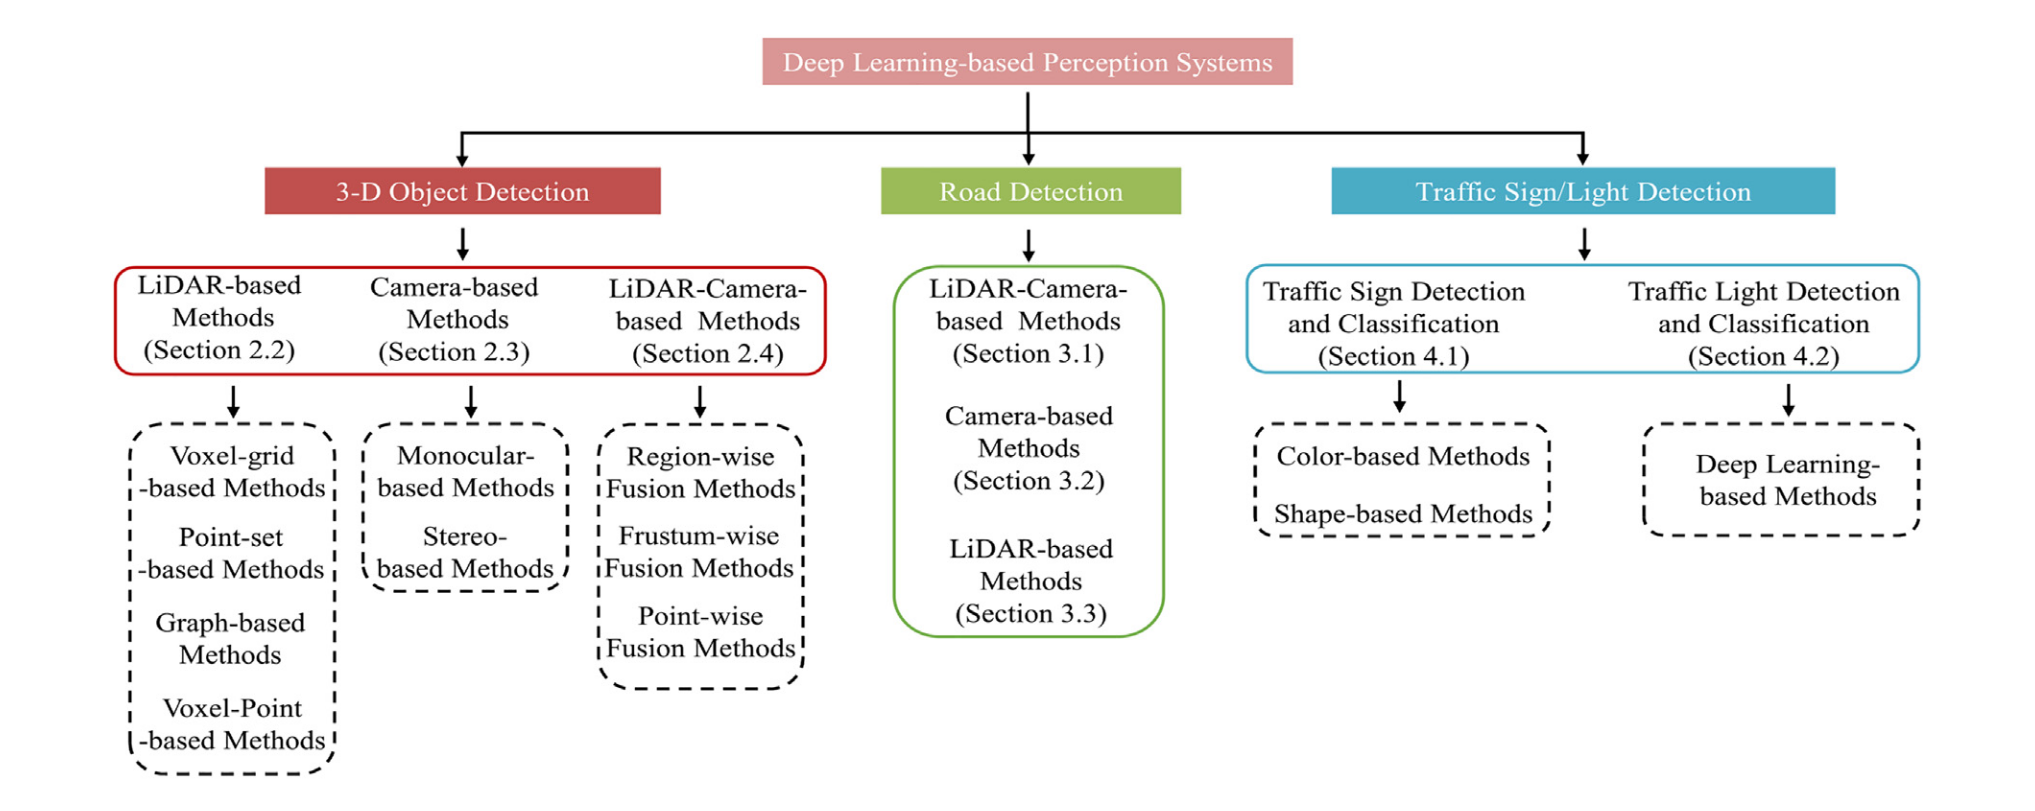
\includegraphics[width=135mm]{figures/learning_based_methods.png}%
  
  \caption{Learning-based perception methods. Source: \cite{learning_based_perception_survey}}%
  \label{fig:learning_based_methods}%
\end{figure}%

Some limitations of learning-based approaches are the need for extensive training data, which can be expensive and time-consuming to collect.
These methods can also struggle to generalize in novel and untrained scenarios, which can be problematic in safety-critical situations where the 
vehicle must make quick decisions based on the perceived environment.

\subsubsection{Deterministic Approaches}

Deterministic approaches use mathematical models to estimate the state of the objects in the scene. 

\paragraph{Optical flow}

Optical flow is a technique used to estimate the motion of objects in the scene by tracking the movement of pixels between consecutive frames.
This method is based on the assumption that the intensity of a pixel remains constant over time, which allows the system to track the movement
of objects based on the changes in pixel intensity \cite{optical_flow_estimation_survey}. Some of the most common optical flow algorithms are the 
Lucas-Kanade method \cite{flow_lucas_kanade} and the Horn-Schunck method \cite{flow_schunck}.


\paragraph{6D Vision}

6D vision is a deterministic perception framework that combines stereo vision and motion tracking to estimate the 3D position and velocity
of objects in the scene. Originally introduced by Franke et all \cite{6d_vision_daimler} this method provides a direct
motion estimation without requiring object segmentation. The key principles of 6D Vision are: 

\begin{enumerate}
  \item \textbf{Stereo disparity estimation:} Calculate the disparity between corresponding points in the stereo images to estimate the depth of objects in the scene.
  \item \textbf{Optical flow tracking:} Track the movement of feature points in the scene between consecutive frames.
  \item \textbf{Kalman filtering:} Use Kalman filters to estimate the 6D state vector (position and velocity) of the feature points in the scene.
\end{enumerate}




\subsection{State of the Art in the FTM}

The Institute of Automotive Technology (FTM) at the Technical University of Munich has conducted extensive research in
 the field of environment perception for autonomous vehicles. This section provides an overview of previous work carried 
 out at the FTM, particularly regarding the perception algorithms, sensor setups, and real-world testing platforms that 
 have contributed to the advancement of autonomous driving research.

\subsection{EDGAR Research Vehicle}

The EDGAR (Excellent Driving Garching) research vehicle is a state-of-the-art autonomous driving platform 
developed at FTM \cite{edgar_hardware}. It serves as a testbench for autonomous driving research, including perception, planning, control, 
and sensor fusion. The vehicle is equipped with a multi-sensor setup, comprising:

\begin{enumerate}
  \item \textbf{Stereo and monocular cameras:} For image-based perception and object detection
  \item \textbf{LiDAR sensors:} For 3D mapping and obstacle detection
  \item \textbf{Radar sensors:} For object avoidance and velocity estimation
  \item \textbf{GPS/IMU:} For localization and motion tracking
\end{enumerate}

\begin{figure}[htb]%
  \centering%
  \begin{minipage}{0.3\textwidth}
    \centering
    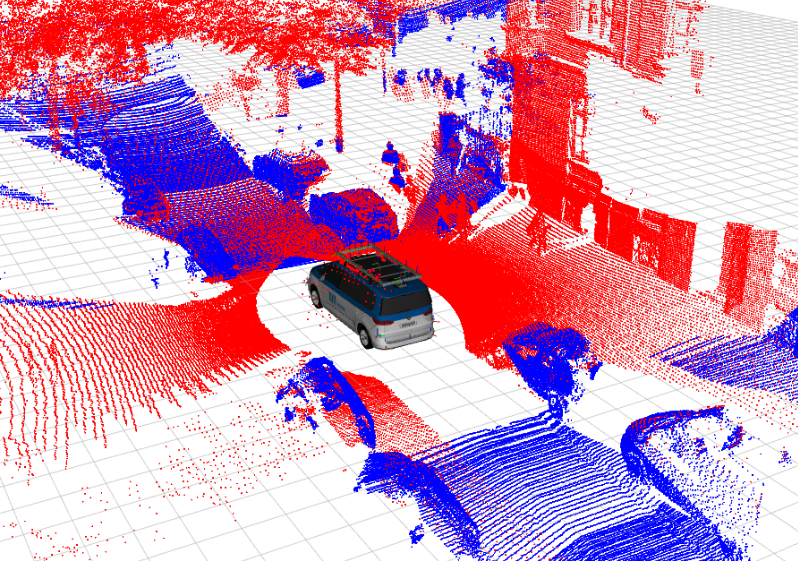
\includegraphics[width=\textwidth]{figures/edgar_3d.png}
  \end{minipage}\hfill
  \begin{minipage}{0.6\textwidth}
    \centering
    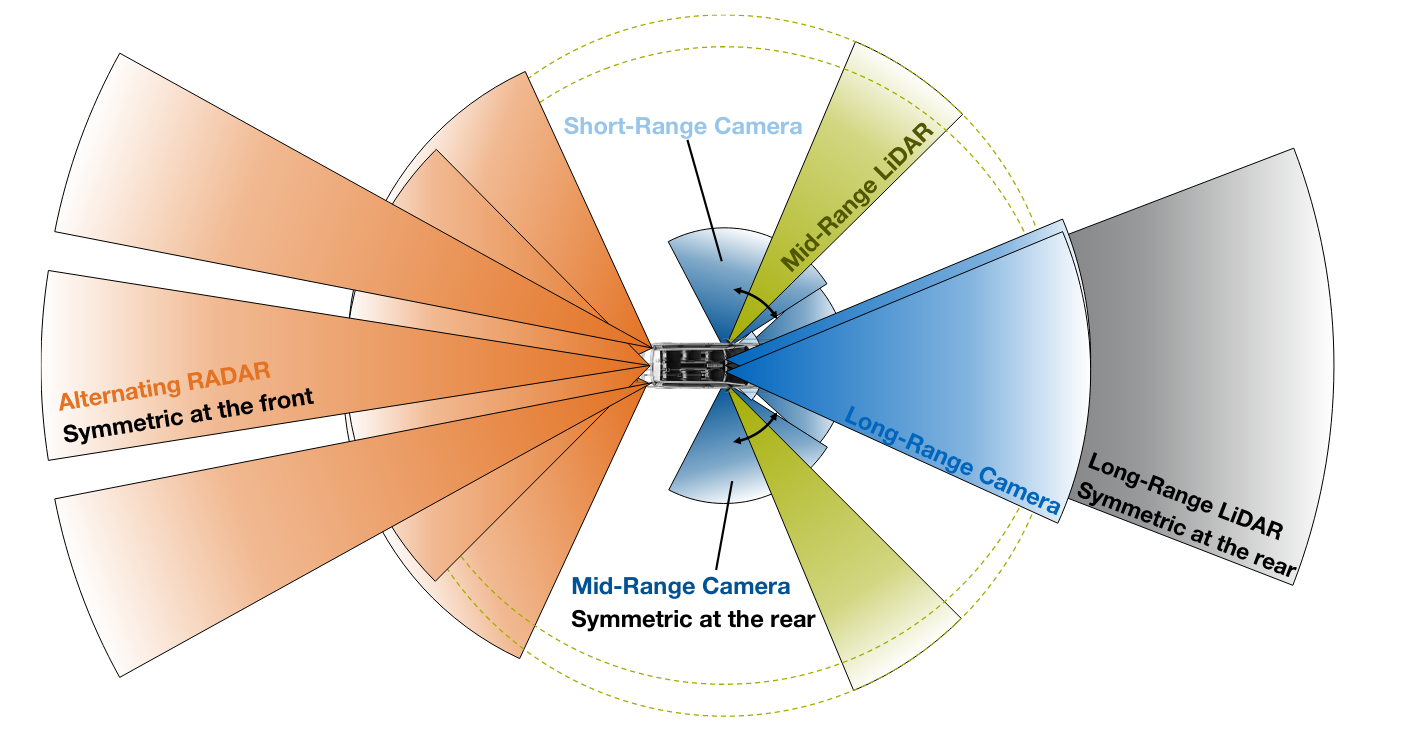
\includegraphics[width=\textwidth]{figures/edgar_sensors.png}
  \end{minipage}
  \caption{EDGAR Vehicle Sensors}
  \label{fig:edgar}%
\end{figure}%



\subsection{Previous Work in the FTM}

This project builds upon previous work conducted at the FTM in the field of environment perception 
for automated vehicles with 6D vision. Some of the key contributions include: 

\begin{enumerate}
  \item \textbf{Objektdetektion und Bewegungsprädiktion mittels eines Stereokamerasystems beim teleoperierten Fahren} \cite{previous_tfm_bauer}: Bauer 
  in his master's thesis developed a deterministic system for object detection based on the 6D vision of Daimler \cite{6d_vision_daimler}. The system 
  was implemented in C++ using the ADTF framework {Automotive Data and Time-Triggered Framework} and was capable of detecting and tracking objects in the vehicle's surroundings 
  with some real time limitations.

  \item \textbf{Weiterentwicklung und echtzeitfähige Umsetzung eines Stereo-Vision-basierten Bewegungsprädiktionssystems für die aktive Sicherheit von teleoperierten Fahrzeugen}
  Some time later in \cite{previous_tfm_gpu_implementation} Rotar continued Bauers work by implementing the system in GPU using CUDA to speed up the computationally intensive tasks.

  \item \textbf{Validation of an Obstacle Detection Approach for Teleoperation of Automated Vehicles:} Finally Pastor \cite{previous_tfm_pastor} started porting the system to ROS1
   to facilitate the integration with other modules in the EDGAR vehicle. The system was implemented without CUDA GPU acceleration
   and was not deployed in the EDGAR vehicle. The system also has some problem with the object detection.
\end{enumerate}

Building upon these previous contributions, this thesis aims to further improve deterministic perception by 
addressing key limitations found in prior implementations. 
In particular, this work will focus on enhancing computational efficiency, real-time feasibility, 
and system deployment within ROS2. These improvements will be detailed in the next section on objectives.






\section{\FTMlangGerEng{Lösungsansatz}{Objective}}%


The goal of this thesis is to develop a deterministic system that can provide a realiable object detection
of moving objects in the ego vehicle's surroundings using stereo camera images and the 6D vision concept.
For this purpose, the work will be devided in two principal pipelines: the perception pipeline 
and the criticality assessment pipeline.

\subsection{Perception Pipeline}%

The perception pipeline will be responsible for detecting the moving objects and outputting 
a list with their position and current velocity. This pipeline will be composed by several submodules as shown in figure \ref{fig:perception_pipeline_high_level}.

\begin{figure}[htb]
  \centering
  \resizebox{0.8\textwidth}{!}{

\begin{tikzpicture}[node distance=0.5cm and 2cm, auto]

  % Primera fila: óvalos de entrada (fuera del contenedor, en azul claro)
  \node[draw, ellipse, fill=blue!20] (params) {Left cam. parameters};
  \node[draw, ellipse, fill=blue!20, right=3cm of params] (limg) {Left image};
  \node[draw, ellipse, fill=blue!20, right=3cm of limg] (rimg) {Right image};

  % Segunda fila: rectángulos de cómputo (dentro del contenedor, en verde)
  \node[draw, rectangle, fill=green!20, minimum width=3cm, minimum height=1cm, below=0.7cm of params] (optflow) {Optical flow computation};
  \node[draw, rectangle, fill=green!20, minimum width=3cm, minimum height=1cm, below=0.7cm of limg] (visodom) {Visual odometry computation};
  \node[draw, rectangle, fill=green!20, minimum width=3cm, minimum height=1cm, below=0.7cm of rimg] (depth) {Depth computation};
  
  % Flechas desde la primera fila a la segunda
  \draw[->, thick] (limg) -- (optflow);
  \draw[->, thick] (limg) -- (visodom);
  \draw[->, thick] (params) -- (visodom);
  \draw[->, thick] (limg) -- (depth);
  \draw[->, thick] (params) -- (depth);
  \draw[->, thick] (rimg) -- (depth);

  % Tercera fila: óvalos de salida de los cómputos (dentro del contenedor, en amarillo claro)
  \node[draw, ellipse, fill=yellow!20, below=0.5cm of optflow] (oflow) {Opt. flow image};
  \node[draw, ellipse, fill=yellow!20, below=0.5cm of visodom] (vo) {Visual odometry};
  \node[draw, ellipse, fill=yellow!20, below=0.5cm of depth] (dimage) {Depth image};
  
  % Flechas desde los rectángulos a los óvalos correspondientes
  \draw[->, thick] (optflow) -- (oflow);
  \draw[->, thick] (visodom) -- (vo);
  \draw[->, thick] (depth) -- (dimage);
  
  % Cuarta fila: kalman filter (rectángulo, dentro del contenedor, en verde)
  \node[draw, rectangle, fill=green!20, minimum width=3cm, minimum height=1cm, below=0.5cm of vo] (kalman) {6D Kalman Filter algorithm};
  
  % Flechas desde los óvalos de salida a kalman filter
  \draw[->, thick] (oflow) -- (kalman);
  \draw[->, thick] (vo) -- (kalman);
  \draw[->, thick] (dimage) -- (kalman);
  
  % Flecha curvada desde "left camera parameters" a "kalman filter"
  \draw[->, thick] (params.south east) .. controls +(1.5, -0.5) and +(-1.5, 0.5) .. (kalman.north west);
  
  % Quinta fila: óvalo "6d image" (dentro del contenedor, en amarillo claro)
  \node[draw, ellipse, fill=yellow!20, below=0.5cm of kalman] (sixd) {6D image};
  \draw[->, thick] (kalman) -- (sixd);
  
  % Sexta fila: rectángulo "Clustering" (dentro del contenedor, en verde)
  \node[draw, rectangle, fill=green!20, minimum width=3cm, minimum height=1cm, below=0.5cm of sixd] (clustering) {Clustering algorithm};
  \draw[->, thick] (sixd) -- (clustering);
  
  % Detected objects: óvalo fuera del contenedor (en azul claro), ubicado abajo
  \node[draw, ellipse, fill=blue!20, below=0.7cm of clustering] (detected) {Detected objects};
  \draw[->, thick] (clustering) -- (detected);
  
  % Contenedor: agrupa los nodos del pipeline (excepto la primera fila y "detected objects")
  \node[draw, dotted, inner sep=0.5cm, fit=(optflow) (visodom) (depth) (oflow) (vo) (dimage) (kalman) (sixd) (clustering)] (perception) {};
  \node[anchor=south east, inner sep=2mm] at (perception.south east) {perception pipeline};
  
\end{tikzpicture}}
  \caption{High level perception pipeline}
  \label{fig:perception_pipeline_high_level}
\end{figure}%

\subsubsection{Optical flow computation}

This module receives as input the left image data from the stereo camera setup and uses it to compute the dense optical flow field.

\subsubsection{Visual odometry computation}

To compute the motion field of the environment, its necessary to know how the ego vehicle is moving with respect 
to the environment.  

Odometry is the use of data from motion sensors to estimate changes in position over time. It is commonly used in 
robotics and autonomous vehicles to track the movement of the vehicle.

Visual odometry, on the other hand, is a specific type of odometry that uses visual data (images or video) to 
estimate the motion of the vehicle. By analyzing the changes in the visual data over time, the system can infer 
the vehicle's movement and position relative to its environment. 
In order to build the pipeline independent of the hardware used, a visual odometry module will 
be implemented to estimate the ego vehicle's motion. 

Visual odometry can be classified into two main categories: monocular and stereo visual odometry.

\begin{itemize}
  \item \textbf{Monocular visual odometry:} Uses a single camera to estimate the motion of the vehicle \cite{vo_mono}.
  \item \textbf{Stereo visual odometry:} Uses a stereo camera to estimate the motion of the vehicle \cite{vo_rev}, including also
  the depth information.
\end{itemize}

Since the system is intended to be used with stereo cameras, and the depth information is already computed for the 
6D vision algorithm, the stereo visual odometry will be implemented.

\subsubsection{Depth computation}

Even through the EDGAR vehicle is equipped with a stereo camera as will be explained in section \ref{subsec:rt_impl},
to ensure the system is robust and can be tested with other camera configurations or datasets, a depth computation module will be implemented
to compute the depth map from the stereo images. This module will take as input the left and right images, as well as the camera calibration
parameters (focal distance, principal point and baseline \cite{pin_hole_camera_model}) and output the depth map of the scene.

\subsubsection{6D Kalman Filter algorithm}

This module will be responsible for estimating the 6D motion of the objects and will serve as the backbone of the perception pipeline.
It will take the dense optical flow field, the depth image and the ego vehicle's motion as input and output the 6D motion of the objects. 
The output will be an image with 6 channels to represent the 6D state of each tracked point in the scene. 
\subsubsection{Clustering algorithm}

To group the 6D motion vectors into objects, a clustering algorithm \cite{clustering_concept} will be implemented. The clustering algorithm will take the 6D motion image as input and output a list of objects with their 6D motion vectors.
For this purpose, the DBSCAN (Density-Based Spatial Clustering of Applications with Noise) algorithm will be used \cite{dbscan_concept}. This clustering
algorithm is suitable for this task since it can handle noise and outliers and does not require the number of clusters to be specified like in 
other clustering algorithms like k-means \cite{kmeans}.

\subsection{Criticality Assessment Pipeline}%

The other pipeline (figure \ref{fig:cp_high_level}) will be responsible for assessing the criticality of the detected objects. This pipeline will be composed
by the criticality algorithm that will compute metrics like the time to collision (TTC) \cite{cricitality_metrics}, based on the object list outputted by the perception pipeline
and the ego vehicle's trayectory. 

\begin{figure}[htb]
  \centering
  \resizebox{0.2\textwidth}{!}{\begin{tikzpicture}[node distance=1.5cm, auto]

  % Nodo de entrada (fuera del contenedor)
  \node[draw, ellipse, fill=blue!20] (detected) {detected objects};
  
  % Nodo del algoritmo (dentro del contenedor)
  \node[draw, rectangle, fill=green!20, minimum width=3cm, minimum height=1cm, below=of detected] (algo) {criticality algorithm};
  
  % Nodo de salida (fuera del contenedor)
  \node[draw, ellipse, fill=blue!20, below=of algo] (metrics) {criticality metrics};
  
  % Flechas de conexión
  \draw[->, thick] (detected) -- (algo);
  \draw[->, thick] (algo) -- (metrics);
  
  % Contenedor punteado que engloba solo el algoritmo
  \node[draw, dotted, inner sep=0.5cm, fit=(algo)] (pipeline) {};
  \node[anchor=south east, inner sep=1mm] at (pipeline.south east) {      criticality pipe.};
  
\end{tikzpicture}}
  \caption{High level criticality pipeline}
  \label{fig:cp_high_level}
\end{figure}%


\subsection{Development and real time implementation}%
\label{subsec:rt_impl}

For the development of the system, the stereo camera setup of front of the EDGAR vehicle will be used. This consist in two Framos D455e stereo 
cameras, two long range Basler cameras in stereo configuration and three medium range Basler cameras for object detection.
These can be seen in the following figure:  

\begin{figure}[htb]
  \centering
  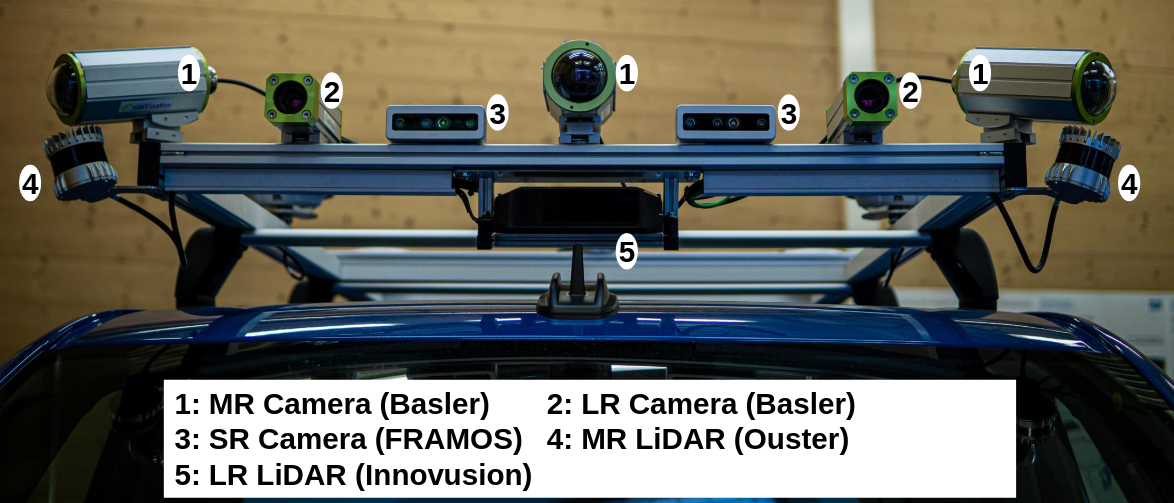
\includegraphics[width=0.8\textwidth]{figures/edgar_visual_perception_sensorkit.png}
  \caption{EDGAR vehicle camera setup}
  \label{fig:edgar_cameras}
\end{figure}%

From this setup, only the Framos and the long range basler cameras will be considered since they are the ones that provide the stereo images.

Regarding the software implementation, the system will be developed in the Robot Operating System (ROS) framework \cite{ros_docu} due to its modularity and seamless integration with the EDGAR vehicle’s existing software. This framework supports two primary programming languages: C++ and Python. Since C++ offers higher performance, it will be used to implement the system.

The EDGAR vehicle employs an architecture based on Docker images for each service. Docker is a platform that automates the deployment of 
applications within lightweight, portable containers. These containers bundle an application together with all its dependencies, libraries, 
and configuration files, ensuring consistent behavior across different environments. 
Consequently, the system must also be containerized using Docker for deployment in the vehicle.

Regarding the real-time implementation, extensive image processing makes a multi-threaded system essential. 
One of the most powerful tools for this purpose is NVIDIA’s CUDA \cite{cuda_concept}, an API that allows the GPU to be used for 
general-purpose computing rather than just image rendering. This capability can be tapped either by writing custom 
CUDA kernels \cite{cuda_kernels} or by using libraries like OpenCV \cite{cervera_gpu_opencv} that include GPU support. 
Consequently, GPU acceleration will be considered 
for all computationally intensive tasks such as optical flow, clustering, and depth computation.


\subsection{Evaluation}%


For the evaluation, two aspects will be assessed separately: the individual components of the perception pipeline and the integrated system.

To evaluate the optical flow, depth computation, and visual odometry modules, the corresponding datasets from the KITTI 
(Karlsruhe Institute of Technology and Toyota Technological Institute) Vision Benchmark Suite \cite{kitti_dataset} will be used. 
These datasets provide a diverse range of real-world driving scenarios—including urban and highway scenes—along with ground truth data 
for optical flow \cite{kitti_flow_article}, depth \cite{kitti_depth}, and visual odometry \cite{kitti_odom}.

To assess the integrated system, the goal is to compare its performance with the state-of-the-art learning-based perception systems 
currently deployed in the EDGAR vehicle. For this purpose, the developed system will be installed on the EDGAR platform and tested 
in various environments, such as urban settings and parking lots. In each scenario, the criticality metrics produced by the system 
will be compared with those generated by the existing perception solutions.

In addition to evaluating output data, another key metric will be the system’s computational time. 
Specifically, the frame rate of each module will be measured, and the overall frame rate of the system will be calculated. 
This is crucial because the system is intended for real-time operations, where low computational overhead is n
ecessary to maintain the required frame rate. These measurements will then be compared with those of the current perception 
systems used in the EDGAR vehicle.

\subsection{Expected Results}%

To summarize the anticipated outcomes of this thesis and how they will advance the department’s ongoing work, the following results are expected:

\begin{itemize} 
  \item Development of a deterministic, 6D vision-based perception system for moving object detection on autonomous vehicles. 
  \item Implementation in C++ using the ROS framework, with containerization via Docker for streamlined deployment on the EDGAR vehicle. 
  \item Integration of GPU acceleration through CUDA, leveraging the work of \cite{previous_tfm_pastor} to improve performance in computationally intensive tasks. 
  \item Capability to estimate criticality metrics, such as time to collision (TTC), for identified objects. 
  \item Evaluation of individual modules using the KITTI dataset and validation of the integrated system on the EDGAR vehicle. 
  \item Enhancement of the existing clustering method by employing the DBSCAN algorithm for more robust object detection. 
\end{itemize}

\section{\FTMlangGerEng{Arbeitsplan und benötigte Ressourcen}{Workplan}}%



In the following sections, the work plan for the thesis is presented. The work plan is divided into five main
work packages (WPs), each with a set of tasks and deliverables. This are:

\begin{itemize}
  \item \textbf{WP1: Literature research and planning:} This WP comprises all the tasks
   that are necessary to understand the state-of-the-art of the frame of the project and 
   learn everything that is necessary to develop the necessary algorithms. It also includes
   the planning phase of the project.

  \item \textbf{WP2: Development of the perception pipeline:} This WP is dedicated to the development,
  fine-tuning and testing of the perception pipeline, which is responsible for detecting the moving objects in the scene.

  \item \textbf{WP3: Development of the criticality assessment pipeline:} This WP is dedicated to the development,
  fine-tuning and testing of the criticality assessment pipeline, which is responsible for assessing the criticality of the detected objects.
  \item \textbf{WP4: Evaluation and discussion of the result:} This WP is dedicated to the deployment of the developed system on the EDGAR vehicle
  and the evaluation of the results. The results will be compared against the state-of-the-art learning-based perception systems currently used in the vehicle.
  For this will be necessary to collect data from the vehicle and analyze it. 
  \item \textbf{WP5: Materthesis project management:} This WP is dedicated to the management of the masterthesis project. It includes the writing of the thesis, the preparation of the presentation and the final defense of the thesis.

\end{itemize}

In the figure \ref{fig:timeschedule} the time schedule of the project is presented as an Gantt Diagram.
\begin{figure*}[htb]%
  \hspace*{-2.5cm} % Adjust the value as needed to move the figure to the left
  \FTMlangGerEng{\input{figures/zeitplan.tikz}}{\begin{ganttchart}[%
	y unit chart=.7cm,%
	canvas/.append style={fill=none, draw=black!5, line width=.75pt},%
	hgrid style/.style={draw=black!5, line width=.75pt},%
	vgrid={*1{draw=black!5, line width=.75pt}},%
	title/.style={draw=none, fill=none},%
	title label font=\bfseries\footnotesize,%
	%title label node/.append style={below=5pt},%
	include title in canvas=false,%
	bar height=0.3,%
	bar label font=\mdseries\footnotesize\color{black!70},%
	bar label node/.append style={left=0.2cm},%
	bar/.append style={draw=none, fill=TUMBlue4},%
	group height=0.3,%
	group label node/.append style={left=0.2cm},%
	group label font=\bfseries\small\color{black},%
	group/.append style={draw=none, fill=TUMBlue},%
	]{1}{24}%
	\gantttitle[title label node/.append style={below left=7pt and 10pt}]{Month}{1}%
	\gantttitlelist[title label node/.append style={below left=7pt and 10pt}]{1,...,6}{4} \\%
	\ganttgroup{\textbf{WP1:} Literature research and planning}{1}{4} \\%
	\ganttbar{Research general perception techniques and paradigms}{1}{2} \\%
	\ganttbar{Research classical methods for environment perception}{1}{2} \\%
  \ganttbar{Research actual requirments in automated vehicles}{2}{4} \\%
  \ganttbar{Research on previous work in the department}{2}{4} \\%
  \ganttbar{Plan how to implement the selected algorithms}{2}{5} \\%
	\ganttgroup{\textbf{WP2:} Perception pipeline development}{5}{13} \\%
	\ganttbar{Collect test datasets}{5}{6} \\%
  \ganttbar{Prepare docker environment}{5}{6} \\%
  \ganttbar{Implement stereo vision package}{6}{8} \\%
  \ganttbar{Implement optical flow package}{6}{8} \\%
  \ganttbar{Implement 6D Kalman Filter}{8}{12} \\%
  \ganttbar{Implement clustering algorithm}{11}{13} \\%
	\ganttgroup{\textbf{WP3:} Criticality pipeline development}{13}{19} \\%
	\ganttbar{Prepare docker environment}{13}{14} \\%
	\ganttbar{Implement criticality metrics pipeline}{13}{19} \\%
	\ganttgroup{\textbf{WP4:} Evaluation and discussion of results}{15}{22} \\%
	\ganttbar{Deploy system on edgar vehicle}{15}{16} \\%
	\ganttbar{Collect data from the vehicle}{17}{18} \\%
  \ganttbar{Analyze the collected data}{18}{22} \\%
	\ganttgroup{\textbf{WP5:} Masterthesis project management}{6}{24} \\%
  \ganttbar{Dissertation writing}{6}{24} \\
  \ganttbar{Preparing presentation}{24}{24}%

\end{ganttchart}%
}%
  \caption{\FTMlangGerEng{Zeitplan}{Time schedule}.}%
  \label{fig:timeschedule}%
\end{figure*}%

